\documentclass{article}
\usepackage{iko42360}
\usepackage{graphicx} % for pdf, bitmapped graphics files
\graphicspath{{./fig/}}
\DeclareGraphicsExtensions{.pdf,.jpeg,.png}
\usepackage{subfigure}
\usepackage[us,12hr]{datetime} % `us' makes \today behave as usual in TeX/LaTeX

\begin{lecture}{3++}{Velocity Motion and Feature-based Measurement Models}{Vektor Dewanto}{05/28/2014}

\section{Introduction}
This lecture note presents two subtopics, i.e. the velocity motion model and the feature-based measurement model.
Feel free to discuss more with the TAs.

\section{Velocity Motion Model}
For robots that offer a velocity control interface, namely: a rotation velocity~$\omega_t$ and a translation velocity~$v_t$, the control $u$ can be expressed in the form of $u = [v_t~\omega_t]^T$.
As a result, for such robots, we may build velocity motion models, instead of odometry motion models.
Notice that the velocity motion model is less accurate than the odometry motion model.
One reason for this is because the odometry is measured by simply counting the encoder's ticks, while the velocity is with the same counting but over some amount of time; the timing here is susceptible to error.
The odometry motion model, however, can not be used for \emph{accurate} planning since it lacks the specification for the duration of execution.

The algorithm for sampling motions using the velocity motion model is shown in figure~\ref{fig:sample_motion_model_velocity}.
In line 2, 3 and~4, the term $sample(\lambda)$ generates a random sample from a gaussian distribution $\mathcal{N}(\mu=0, \sigma= \lambda)$. 
Meanwhile, the term~$\hat{\gamma}$, which firstly appears in line~4, denotes a random noise in the final orientation.
There are six intrinsic parameters, i.e. $\{\alpha_i\}_{i=1}^6$, which are robot-specific.
We remark that the duration~$\triangle t$ in line 4, 5 and~6 is typically a constant. 

\begin{figure}[!b]
  \centering
  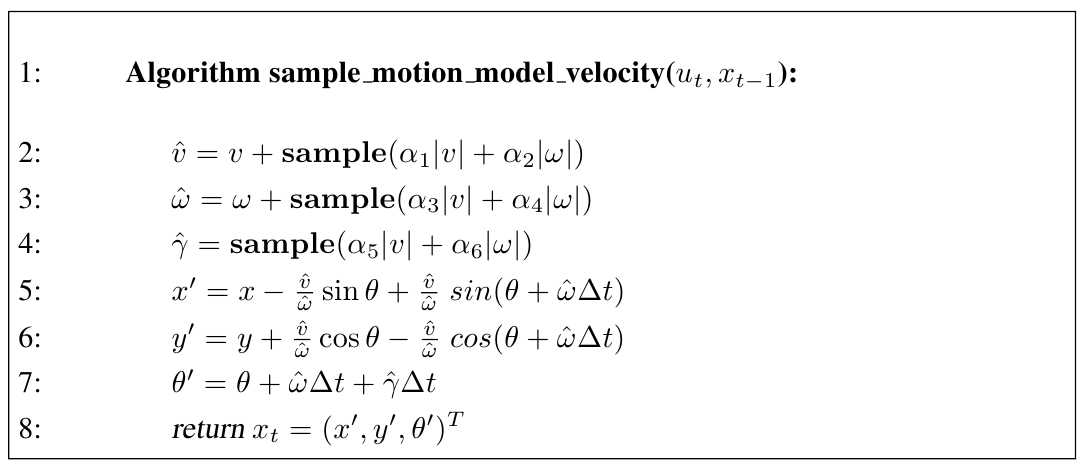
\includegraphics[scale=.5]{sample_motion_model_velocity}
  \caption{The algorithm for sampling motions using the velocity motion model; courtesy of~\cite{Thrun:2005:PR}.}
  \label{fig:sample_motion_model_velocity}
\end{figure}

\section{Feature-based Measurement Model}
The beam-models for range finders utilize raw measurements from, for example, sonars.
In some cases, however, we have the luxury of sensors that, at time~$t$, return a set of features~$\{f_t^i\}$ extracted (hence, having much fewer dimensions) from raw measurements.
Furthermore, let $c_t^i$ denotes a correspondence variable between a feature~$f_t^i$ and the landmark~$m_j$ in the map~$m$, such that $c_t^i \in \{1, 2, \ldots, N\}$, where $N$ is the number of landmarks.
Recall that in a landmark-based map, a map~$m$ is represented as a list of landmark coordinates, i.e. $m = \{m_i\}_{i=1}^N$; in a 2D planar world, $m_i = [m_{i,x}~m_{i,y}]^T$.

The algorithm for computing the likelihood of a landmark measurement $p(f_t^i | c_t^i, m, \boldsymbol{x}_t)$ is shown in figure~\ref{fig:landmark_model_known_correspondence}, with $f_t^i = [r_t^i~\phi_t^i~s_t^i]^T$, where $r$, $\phi$ and $s$ denote the range, the bearing and the signature of a landmark, respectively.
Line~3 and~4 calculate the true range and bearing to the corresponding landmark~$m_j$ (as indicated by~$c_t^i$ in line~2) from the current pose~$\boldsymbol{x}_t = [x~y]^T$.
Afterward, the probability of the measured range and bearing is calculated in line~5, in which we model the noise in landmark perception by independent Gaussian noise with $\mu=0$ and $\sigma_r$, $\sigma_{\phi}$, $\sigma_s$ for the measurements of $r_t^i$, $\phi_t^i$ and $s_t^i$, respectively.
Notice that $r$ and $\phi$ are continuous values, hence they have probability density functions.
\begin{figure}[!tb]
  \centering
  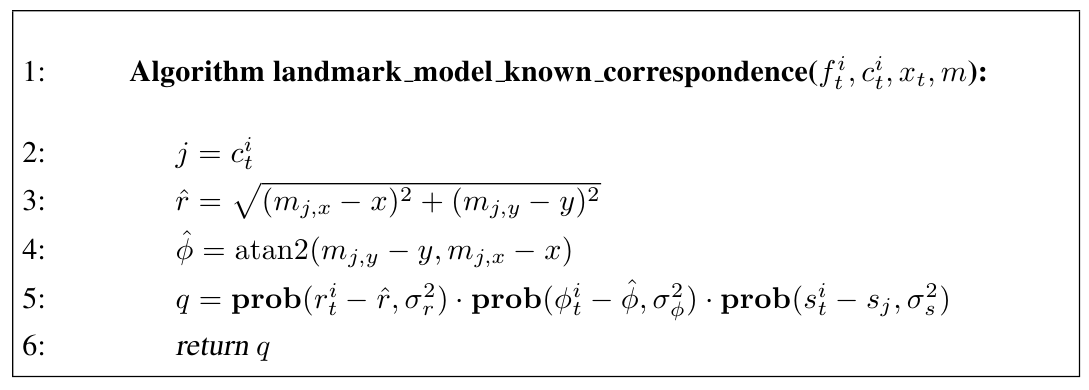
\includegraphics[scale=.5]{landmark_model_known_correspondence}
  \caption{The algorithm for computing the likelihood of a landmark measurement; courtesy of~\cite{Thrun:2005:PR}.}
  \label{fig:landmark_model_known_correspondence}
\end{figure}

As a working example, consider a vision system that consists of a gray-scale monocular camera and a processing unit.
In particular, the camera outputs 2D images, whose pixel value is equal to the 8-bit brightness level; say, 0 for black and 255 for white.
The processing unit~$f(z)$ takes as input an image and extracts a feature vector~$f$.
Concretely, $f(z) = [s~r~\phi]^T$, where $s$ contains the measured brightness level of a landmark region in the input image, $r$ and~$\phi$ are the range and the orientation between the robot and the observed landmark, which are inferred from the 2D input image with a sophisticated-yet-erronouos spatial constructor.
Whenever no landmark is on the field of view of the camera, $f(z) = \emptyset$.
Let assume that on our favourite map, there are five landmarks $m_j \in \{A, B, C, D, E\}$ as shown in figure~\ref{fig:map_with_landmark}.
Each landmark has a unique signature based on the brightness level.
For example, the identity of landmark~A is with $s= 25$, eventhough any feature whose $s \in [0,50]$ corresponds to landmark~A.
The position of a landmark is always computed towards its center point.

\begin{figure}[!tb]
  \centering
  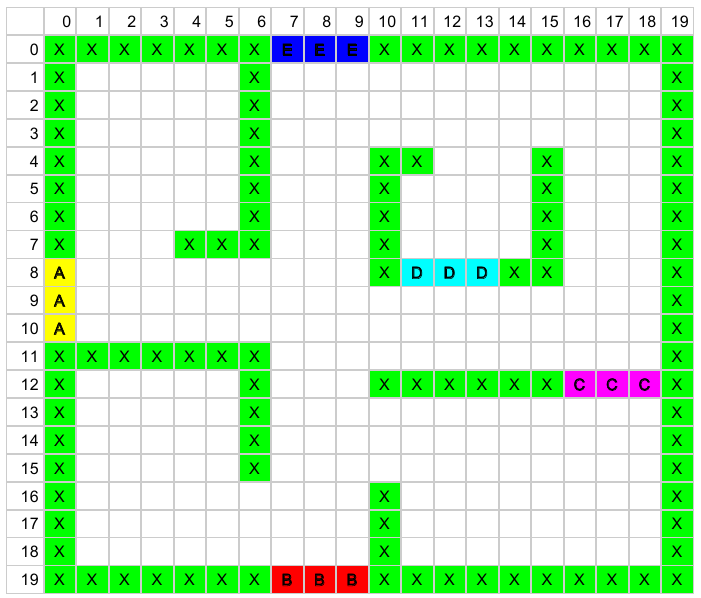
\includegraphics[scale=.7]{map_with_landmark}
  \caption{Our favourite map with five landmarks.}
  \label{fig:map_with_landmark}
\end{figure}

We have to simulate the way the aforementioned vision system works.
One possible approach is as follows.
Use ray-casting to determine whether a landmark is on the field of view of the camera.
If so then the processing unit returns a feature~$f$ that contains three noisy values (may be drawn from a Gaussian distribution).
The corresponding landmark is determined using the (noisy) $s$-component of~$f$.

\section{Miscellany}
(compiled on {\ddmmyyyydate\today} at \currenttime)

\bibliographystyle{IEEEtran}
\bibliography{IEEEabrv,ln}

\end{lecture}
\theend
